\begin{refsection}

\def\chaptertitle{Data legacy}


\chapter[\chaptertitle]{\chaptertitle}
\chaptermark{Data legacy}
\label{ch:legacy}

\clearpage{}
\section{Introduction}
\label{legacy:sec:intro}

In the spirit of expanding the definition of academic success \citep{Goring2014} and fostering open collegiate science \citep{Hampton2015}, this chapter discusses the products of this PhD project outwith the immediate results-based thesis chapters. It is my hope that the data and research infrastructure generated during this PhD will have a legacy beyond the uses I have found for it thus far, providing value to myself as I progress through my academic career, and to other researchers. Specifically, this chapter discusses the extended value of the data collected during the PhD, the steps taken to ensure that data are visible to and usable by other researchers, existing research outputs by colleagues utilising the data, and a non-exhaustive list of future projects which could use the data in novel and impactful ways.

There are two principal non-chapter outputs of this PhD project. Firstly the network of permanent plots and accompanying census data in Bicuar National Park, southwest Angola, and secondly the terrestrial LiDAR data collected in 22 1 ha plots, including all 15 in Bicuar National Park and a further seven in Kilwa District, southern Tanzania.

\section{Permanent plots in Bicuar National Park}
\label{legacy:sec:bicuar}

The 15 1 ha permanent plots in Bicuar National Park were set up in collaboration with Dr. Francisco Maiato Gon\c{c}alves from the Herbarium of Lubango, Hu\'{i}la province, Angola, with the help of a National Geographic Society grant (Grant No. EC-51464R-18). These plots provide not only a valuable dataset of woody stem measurements but also an infrastructure for further ecological research and an opportunity for continued scientific collaboration between the University of Edinburgh and the Herbarium of Lubango.

The Herbarium of Lubango is located \textasciitilde{}300 km from Bicuar National Park. During their installation and in the year after, the plots were used by the Instituto de Ci\^{e}ncias da Educa\c{c}\~{a}o Huila (ISCED), which is partnered with the Herbarium of Lubango, to teach Ecology Masters students about woody biomass estimation techniques and plant taxonomy. As teaching resources at public institutions in Angola can be scarce, our partnership with ISCED provides a clear capacity building benefit that will hopefully strengthen academic interest in woodland monitoring programmes at the institution.

A number of voucher specimens from tagged trees in the plots are held in the Herbarium of Lubango, with duplicates of most currently held in the Royal Botanic Gardens at Kew, London, UK. We hope to conduct more botanical collections during future censuses to update the checklist of plant species found in Bicuar National Park, with the hope of raising the profile of this valuable woodland refuge at the far western extent of the miombo ecoregion, and improving its protection and development as a natural resource by the Angolan government. To this end, in 2019, in addition to setting up the 1 ha permanent plots, we conducted 20 one-off 20x50 m samples of previously abandoned agricultural land at the edge of the park boundaries, to improve our coverage of land-use types in the Park and to better understand the biodiversity recovery of regenerating agricultural landscapes.

Steps have been taken to ensure the longevity of the permanent plots. The value of a plot focussed monitoring programme generally increases over time as more data is accrued and temporal trends can be identified, so efforts must be made to ensure that regular censuses and maintenance are conducted. In 2020 all plot corners were marked permanently with concrete posts (\autoref{legacy:concrete}), and have been located with highly accurate differential-GPS, to an accuracy of $\le$3 cm. Knowing the plot boundaries to a high degree of accuracy will increase their value as plots to be matched with highly precise satellite data products that are currently emerging \citep{Exbrayat2019, GeorgeChacon2019, Wagner2018}. 

Data from the first census of the plots are held in the SEOSAW database \citep{SEOSAW2020}. The SEOSAW database holds standardised woody stem measurements from plots spanning southern Africa. The data in SEOSAW are available to all researchers following agreement by the data holder and all other SEOSAW members. The permanent plots in Bicuar are the most westerly permanent plots in the SEOSAW plot network (\autoref{legacy:seosaw_plots}), occupying a climate space within the region not currently served by other permanent plots (\autoref{legacy:seosaw_clim}). Holding the plot data from Bicuar in SEOSAW also acts as a permanent data backup repository, extending the lifespan of the data.

A second woody stem biomass survey is planned for all plots in 2022/2023, with the aim of improving the quality of data collected and assessing mortality and productivity over time. This re-census will likely happen as part of either the SEOSAW or SECO projects, both operating out of the University of Edinburgh. Data from the second census will be provided to SEOSAW and eventually uploaded along with the first census to ForestPlots.net \citep{LopezGonzalez2011}, increasing visibility of the data further.

\begin{figure}
	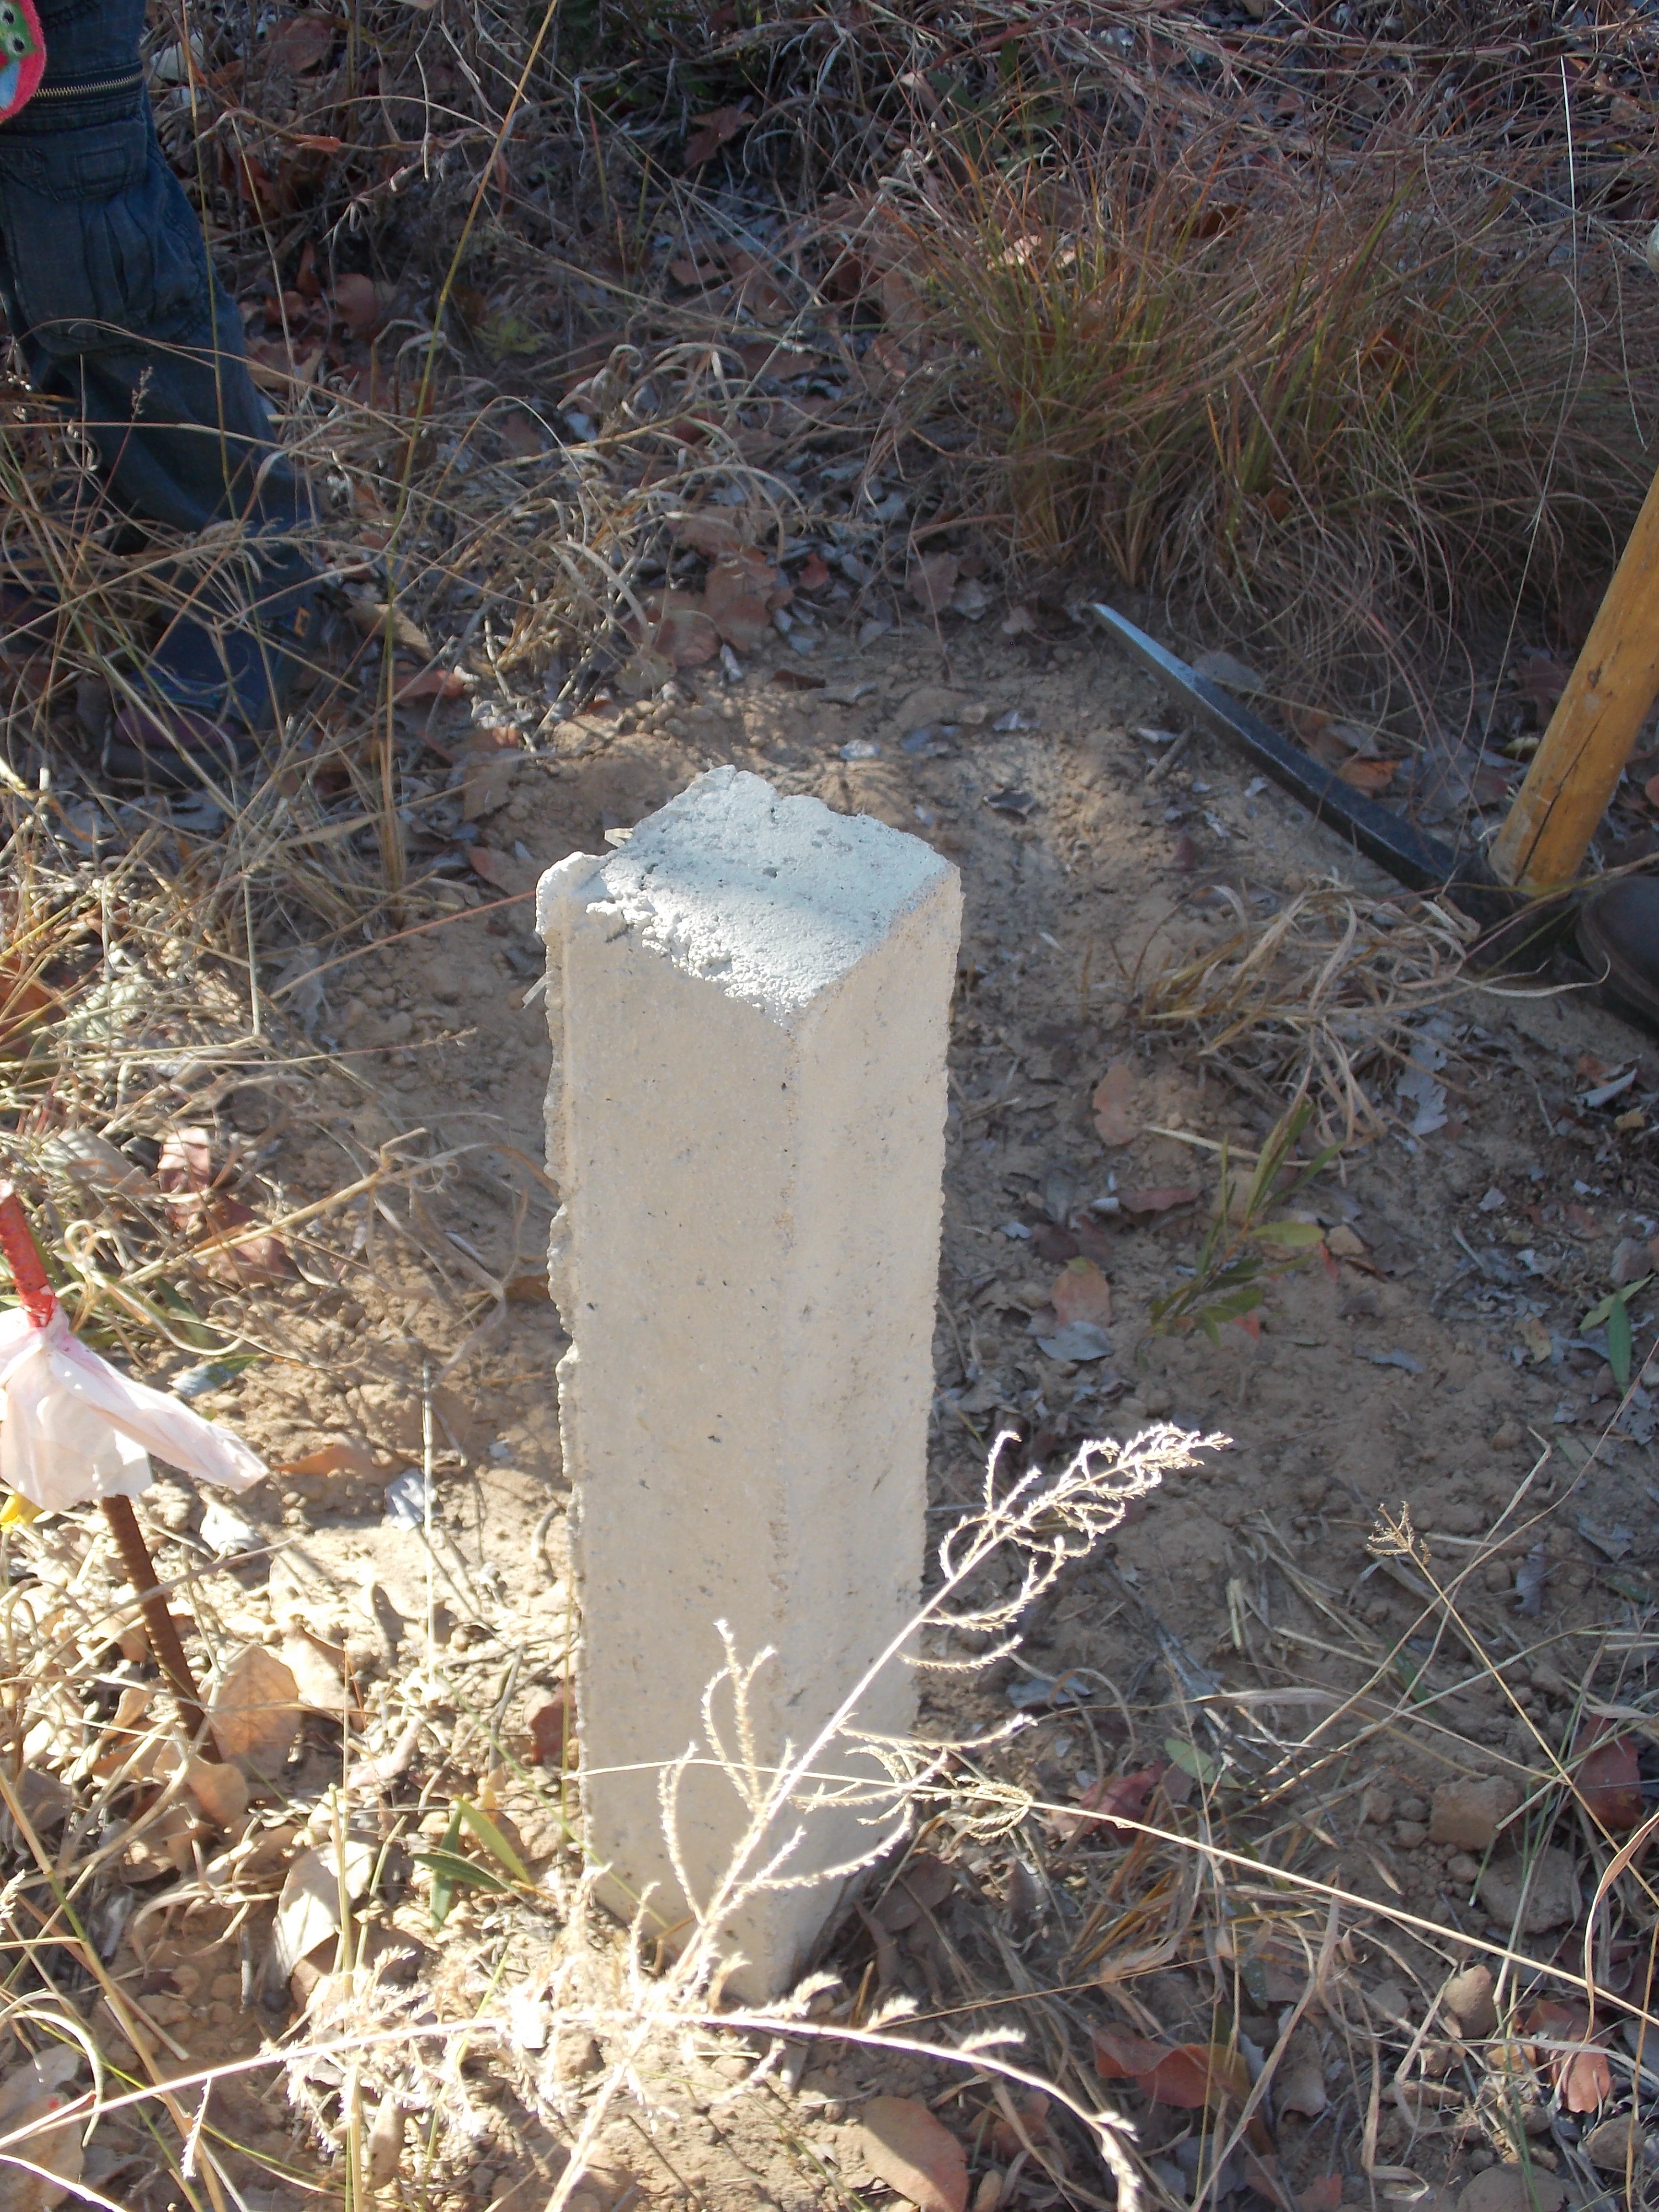
\includegraphics[width=0.6\linewidth]{img/concrete}
	\caption[Concrete corner posts in Bicuar National Park]{An example of the concrete posts installed to a depth of 1 m at the plot corners of all 1 ha plots in
	Bicuar National Park, to ensure that plot boundaries are not lost and do not drift over
repeated censuses.}
	\label{legacy:concrete}
\end{figure}

Data from these plots have already been utilised in four peer-reviewed articles led by colleagues:

\begin{itemize}
	\item{\fullcite{Panzou2020}}
	\item{\fullcite{SEOSAW2020}}
	\item{\fullcite{Silva2020}}
	\item{Esquivel-Muelbert, A. ... (in prep. Nature Communications 2021). Bridging scales in monitoring tree mortality globally.}
\end{itemize}

\begin{figure}
	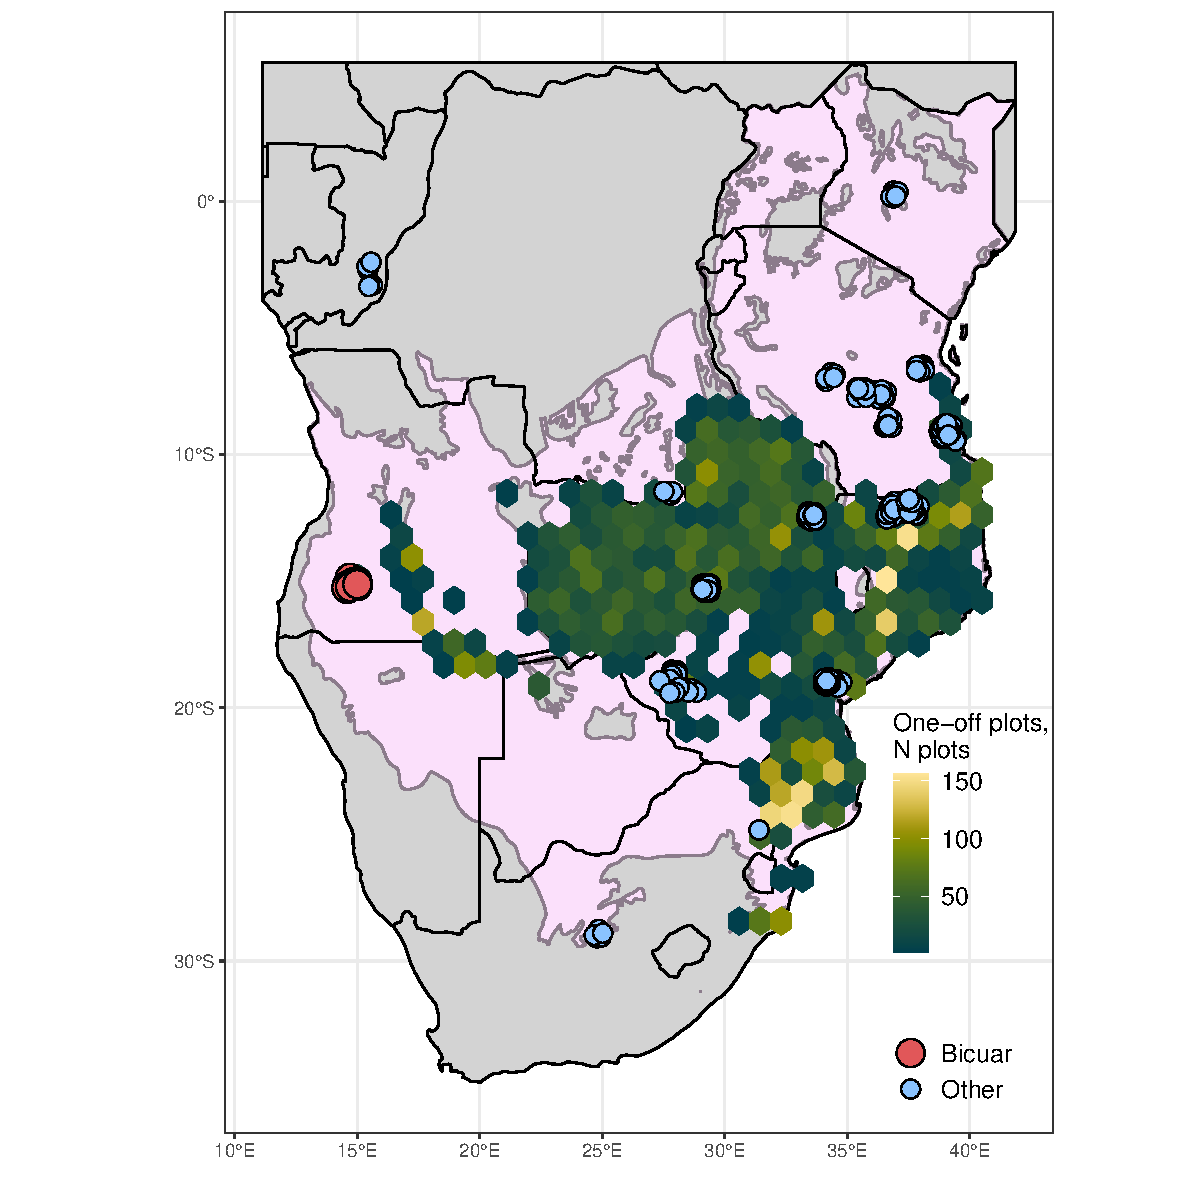
\includegraphics[width=0.8\linewidth]{img/seosaw_plots}
	\caption[Spatial distribution of plots in the SEOSAW network]{The spatial distribution of plots in the SEOSAW network. Blue circles are permanent plots, where individual stems are tagged and can be matched among censuses. The permanent plots in Bicuar National Park are shown as red points. The hexagon grid shows the density of one-off plots.  The pink shading shows the working region of the SEOSAW network, defined primarily from woodland defined by \citet{White1983} and further adapted to bound the north-eastern and southern boundaries.}
	\label{legacy:seosaw_plots}
\end{figure}

\begin{figure}
	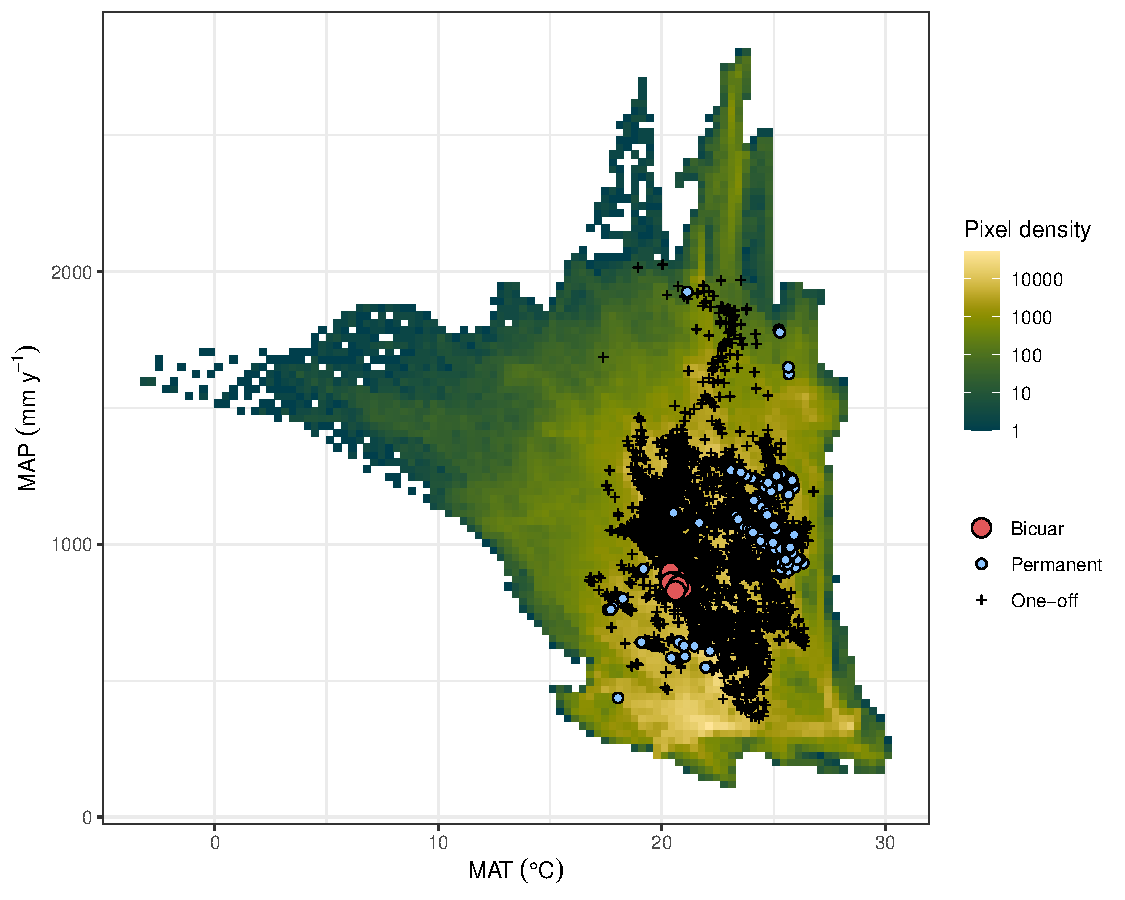
\includegraphics[width=0.8\linewidth]{img/seosaw_clim}
	\caption[Climatic distribution of plots in the SEOSAW network]{The distribution of SEOSAW plots in climate space, using Mean Annual Temperature (MAT) and Mean Annual Precipitation (MAP) from the WorldClim database \citep{Fick2017}. Blue circles are permanent plots, where individual stems can be matched among censuses. The permanent plots in Bicuar National Park are shown as red points. Black crosses show one-off plots. The background is shaded according to the density of pixels in the SEOSAW working region, described in \autoref{legacy:seosaw_plots}.}
	\label{legacy:seosaw_clim}
\end{figure}

\subsection{Bicuar National Park as a `Supersite'}
\label{legacy:ssec:supersite}

There has been a recent push to establish certain long-term ecological monitoring sites as `supersites'. A supersite is defined here as a ``highly-instrumented research site where all ecosystem compartments and fluxes are covered'' \citep{Mikkelsen2013}. Establishment of supersites has been identified as a goal by a number of international projects which seek to improve global land-atmosphere modelling and monitoring of the effects of climate change on ecosystem structure and function. Notable organisations include the Forest Observation System (FOS, \citealt{Chave2019}), and the upcoming SECO project at the University of Edinburgh (NERC Large Grant NE/T01279X/1). The impetus behind the supersite model is that it is more cost-effective to prioritise a small number of sites that are representative of a given landscape's ecology as locations for concentrating multiple expensive measurements, such as LiDAR and atmospheric flux towers. These highly-instrumented sites then form the apex of a hierarchy of sites within the landscape most of which only have limited monitoring measurements. Measurements from the supersites can then be used to `scale up' to the landscape scale with the help of the less-provisioned sites and remotely-sensed data \citep{Anderson2018}. Concentrating multiple measurements within a few sites allows more ready comparison of these measurements, which when scattered among nearby sites can severely decrease their predictive power due to individual site conditions \citep{Mikkelsen2013}.

Some of the common requirements for supersites outlined by various projects have already been fulfilled for the plots in Bicuar National Park. Since 2015, SASSCAL (Southern African Science Service Centre for Climate Change and Adaptive Land Management) has maintained a weather station at Bicuar National Park, providing freely available hourly data on air temperature, solar irradiance, wind speed and direction, soil moisture, precipitation and air pressure \citep{SASSCAL_weather}. The weather station is located within 20 km of all the permanent plots. A critical requirement for a supersite in many projects is that it has a combination of either terrestrial and/or airborne LiDAR measurements. LiDAR provides invaluable information on forest structure that is precisely geo-referenced, helping to bridge the scale gap between ground measurements and satellite measurements. The 15 plots in Bicuar National Park already have a comprehensive terrestrial LiDAR dataset, with precise geo-referencing, collected in 2019. The possibility of repeat LiDAR measurements in combination with an airborne LiDAR campaign would make Bicuar National Park an extremely valuable resource. Additionally, the GEDI L2B satellite LiDAR product has good coverage over Bicuar National Park, with the potential to compare these measurements with the terrestrial LiDAR in the plots (\autoref{legacy:bicuar_tracks}). To our knowledge there are no other plot-based terrestrial LiDAR datasets of dry tropical woodlands in southern Africa. Our hope is that Bicuar National Park can be registered as a supersite with one or more research organisation and become a destination for researchers, strengthening the representation of Angolan science, and advertising Bicuar National Park and the Herbarium of Lubango as a destination for researchers, building capacity, research potential and conservation awareness in the region.

\begin{figure}
	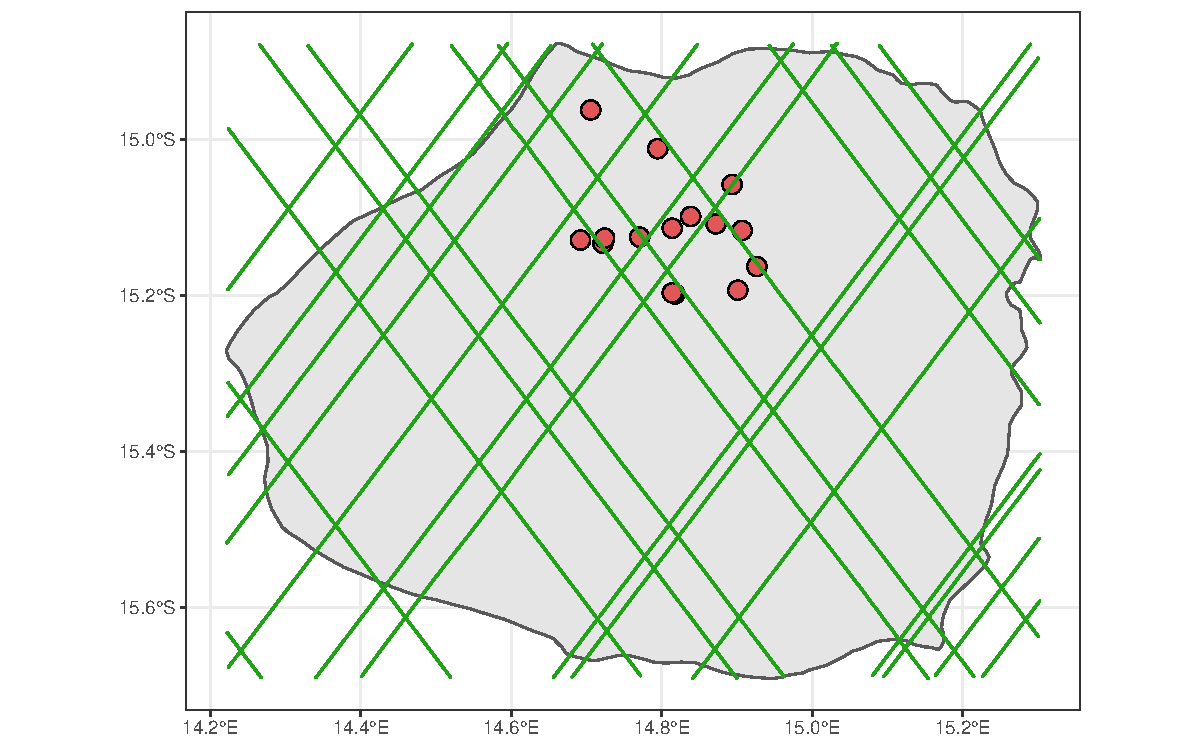
\includegraphics[width=\linewidth]{img/bicuar_tracks}
	\caption[GEDI satellite LiDAR tracks over Bicuar National Park]{50 m wide flight-paths of the GEDI L2B satellite LiDAR product (red lines), with the extent of Bicuar National Park (grey polygon), and the locations of the 15 1 ha permanent plots (blue points). Note that in reality each 25 m track consists of a series of 25 m radius circles which contain LiDAR data.}
	\label{legacy:bicuar_tracks}
\end{figure}

\section{Terrestrial LiDAR}
\label{legacy:sec:lidar}

In addition to the value of terrestrial LiDAR data to qualify as a supersite, as described above, the terrestrial LiDAR data collected as part of this thesis has other uses and values. The LiDAR data has been archived on the University of Edinburgh DataShare, with a permanent DOI (\todo{DOI ID}), along with details of the largely free and open source reproducible workflow for processing the data, which is also seen in Chapter 5 of this thesis. When Chapter 5 is eventually published as a peer-reviewed article, the data repository will be advertised in the article. It is my hope that other researchers will use the data for their own research, extending its lifespan to that which befits the effort expended to collect it. An alternative method to increase visibility of the dataset and encourage its use by others could be to publish an article in a journal like ``\textit{Data in Brief}'', which specialises in short reports on open-access datasets.

The LiDAR data was collected in a way to maximise its potential future uses. The sampling density is sufficient to reliably estimate the canopy height profile of an entire plot, to segment individual trees from the point cloud and to distinguish internal tree canopy architecture. A key application of terrestrial LiDAR is in linking to air- and space-borne LiDAR, and other remotely sensed data products to bridge the scale gap between plot and landscape studies \citep{Xiao2019}. Recent studies have used a combination of terrestrial LiDAR and other remotely-sensed data products to scale up models of functional traits from individual leaves to landscapes \citep{AbelleiraMartinez2016}, calibrate landscape models of biomass distribution \citep{RejouMechain2019}, and infer 3D forest structure with satellite data products \citep{Fischer2020}. My hope is that the LiDAR data may be used by other researchers to answer questions pertinent to the functioning of southern African woodlands. Currently, very few studies using terrestrial LiDAR have been conducted in savannas \citep{Muumbe2021}. In southern African, to my knowledge, all existing studies have been located at Skukuza Flux Tower, Kruger National Park \citep{Singh2018}. Yet, terrestrial LiDAR could provide a useful tool to measure the biomass and physiognomy of shrubs and idiosyncratic trees that comprise a large part of the biomass in these disturbed ecosystems \citep{Muir2018}. The data collected during this thesis therefore make an important contribution to the field of savanna ecology, and by making the data available to other researchers I hope to raise the profile of TLS as a tool for savanna ecology. The following sections contain justifications for future studies I wish to undertake personally using the data collected during this project.

\subsection{Tree taper modelling from Terrestrial LiDAR} 
\label{legacy:ssec:taper}

The most common way of assessing aboveground woody biomass of trees is through allometric models which estimate biomass from a combination of stem diameter, tree height and wood density \citep{Chave2014}. These allometric models often assume that stem diameter is measured at a height of 1.3 m, a convention that is widely followed across forestry and ecology \citep{Brokaw2000}. Peculiarities in stem shape occasionally require the measurement of stem diameter at a different height however, to avoid abnormalities such as burls, fluting, or branch nodes that would otherwise provide an unrepresentative estimate of stem diameter if measured at the conventional height \citep{Kershaw2017}. On average, stem diameter tapers towards the top of a tree \citep{Kozak1969}, meaning that without proper correction, biomass estimates generated from these diameter measurements at unconventional heights will over- or under-estimate biomass. 

Many models of stem taper have been developed, being used by foresters for over a century to estimate harvestable timber volumes, and are still the subject of active development \citep{MacFarlane2016, Luoma2019}. As well as estimating harvestable volume, stem taper models can be used to correct for variation in stem diameter measurement height, to ensure consistent estimates of woody biomass or harvestable volume. Previously these models have been parameterised through multiple measures of stem diameter at different heights with a tape measure, but this is time-consuming and suffers from the same imprecision and human error as any other diameter tape measurement \citep{Saarinen2019}. 

Plot-based estimation of woody biomass across the globe currently relies on measuring stem diameter \citep{SEOSAW2020, Chave2005, Schepaschenko2019}. Being able to accurately reconcile stem diameters measured at different heights is therefore paramount to improving our models of above-ground woody biomass.

Rapid progress has been made in methods to model woody stem diameter from terrestrial LiDAR point clouds \citep{Bogdanovich2021, Hopkinson2004, Srinivasan2015, Ravaglia2019, Wang2016}. These methods estimate a cylinder of the stem from a slice of points, with recent advancements allowing interpolation of the cylinder even when the coverage of laser returns on the stem surface is incomplete. Others have extended the method to generate estimates of stem taper \citep{Henning2006, Thies2004}, but to our knowledge this has not been done for any tree species growing the dry tropics. The terrestrial LiDAR data collected in Angola and Tanzania provide the opportunity to conduct this first study of stem taper from LiDAR measurements in the dry tropics. The species, locations, and stem diameters of all stems >5 cm diameter is known within these plots, meaning that these data can be matched with stems observable in the LiDAR point cloud. As a proof of concept, I have developed a prototype stem segmentation using \texttt{treeseg} \citep{Burt2018}, and a cylinder interpolation method based on \citet{Umbach2003}, which estimates stem diameter at multiple heights along the tree stem (\autoref{legacy:cylinder}).

\begin{figure}
	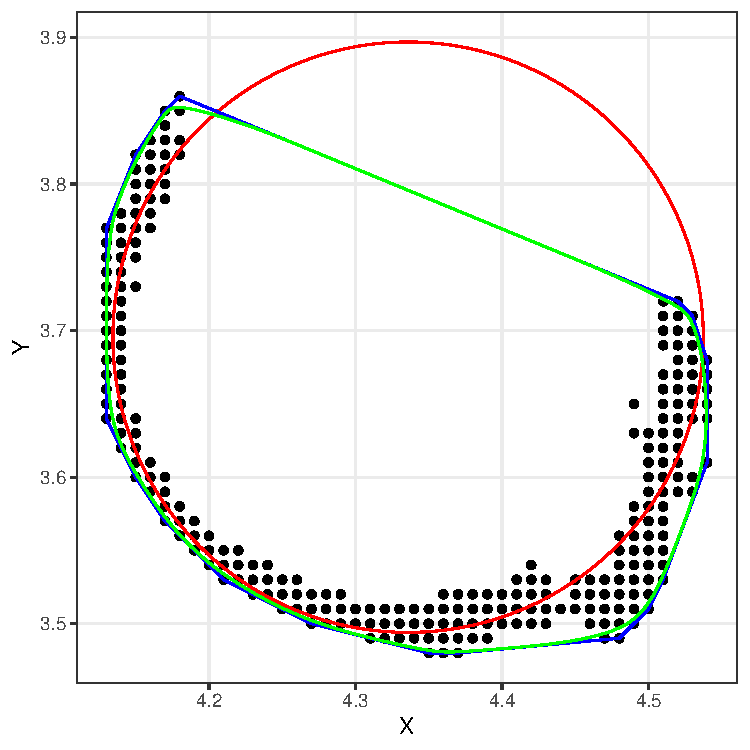
\includegraphics[width=0.6\linewidth]{img/cylinder}
	\caption[Stem cross section cylinder interpolation to estimate stem diameter from terrestrial LiDAR]{Example output of the prototype stem cylinder interpolation method used to estimate stem diameter from an incomplete point cloud. Voxelised points at 2 cm\textsuperscript{3} are shown as black points. Interpolation methods are shown as coloured polygons. The interpolated stem cylinder method based on \citet{Umbach2003} is shown in red. A convex hull of all points is shown in blue. A kernel smoothing method using Gaussian kernel regression is shown in green.}
	\label{legacy:cylinder}
\end{figure}



\subsection{Biomass of large trees: testing scaling theory for estimating biomass}
\label{legacy:ssec:scaling}

Large diameter trees hold a disproportionately large amount of woody biomass in most wooded ecosystems \citep{Bastin2015, Lutz2018}. To accurately describe the woody biomass stocks of a particular system, more effort should therefore be allocated to accurately estimating the biomass of the largest trees. Woody biomass is most commonly estimated through allometric equations which rely on measures of stem diameter, tree height and woody density. At the root of these allometric equations are a limited number of destructive biomass harvests, which define the relationship between tree physiognomic measurements and the biomass of the harvested tree \citep{Chave2005}. Biomass harvesting is time consuming, expensive, and understandably not a popular activity among ecologists due to its destructive nature \citep{Roxburgh2015}. Furthermore, allometric equations are often least well defined for the largest trees, as large trees are scarcer than small trees \citep{Lutz2018, Lindenmayer2012}, and even less likely to be cut down during destructive harvests due to the cultural and aesthetic value they hold as living organisms \citep{Blicharska2014}. Specifically the parameterisation of the exponent term of traditional diameter-biomass allometry power-models is often poor for large trees, and there is a heteroscedastic relationship between diameter and biomass at higher stem diameters (\autoref{legacy:allometry}) \citep{Chave2004, Chave2014}. Recently, the suitability of power-models for diameter-biomass allometries has even been drawn into question, though an alternative that works globally has not yet been found \citep{Picard2015}. Weighting procedures so that large rare trees with higher intrinsic variability in biomass do not overly influence model coefficients have been used successfully previously \citep{Chave2014, McNicol2015b}, but this does not solve the root problem that the biomass of newly encountered large trees will likely be poorly estimated. 

\begin{figure}
	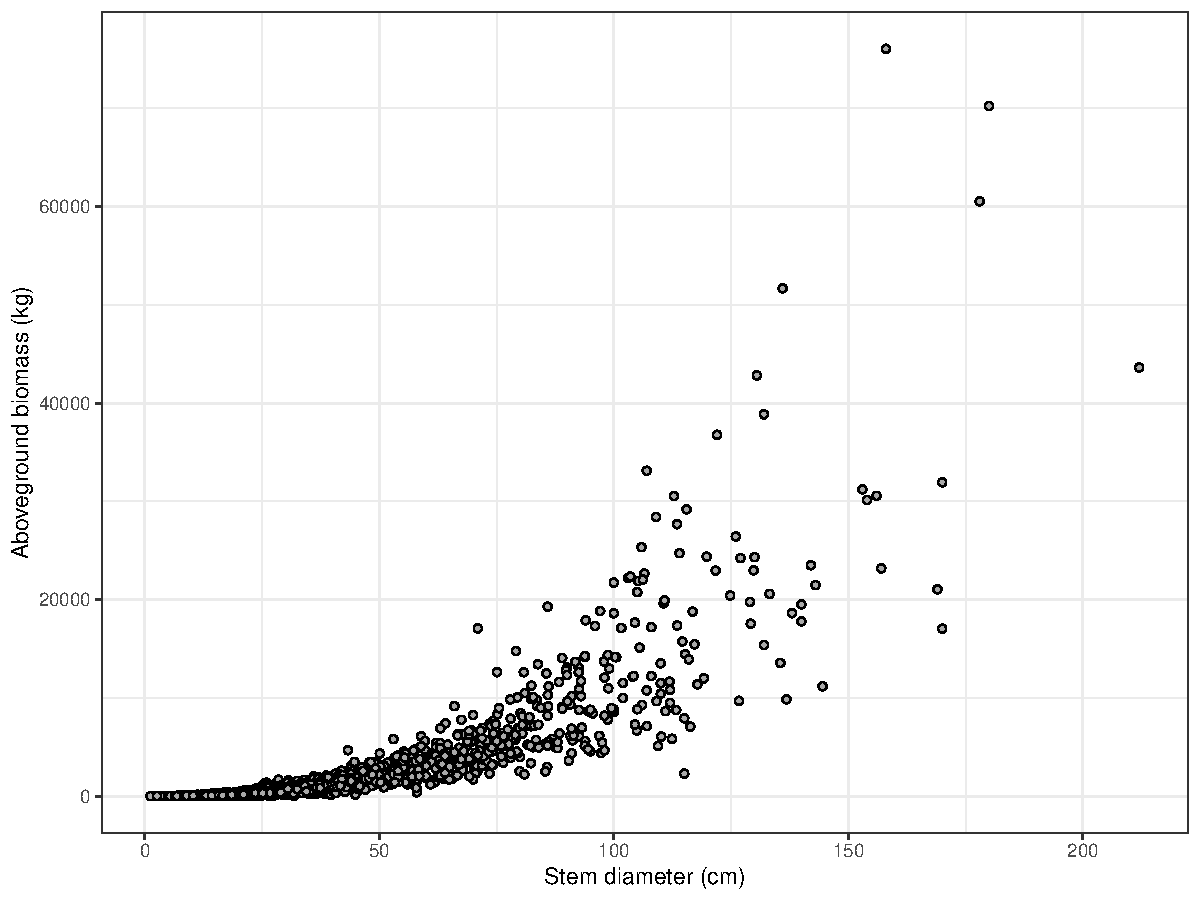
\includegraphics[width=\linewidth]{img/allometry}
	\caption[Scatter plot of stem diameter and biomass from GlobAllomeTree database]{The relationship between tree stem diameter and aboveground biomass calculated from destructive harvest from all 872 records held in the GlobAllomeTree database \citep{Henry2013} and all 4004 records reported in \citet{Chave2014}. The heteroscedasticity of the relationship between stem diameter and aboveground biomass can be seen, with increased variance in biomass at higher stem diameters.}
	\label{legacy:allometry}
\end{figure}

As the age of a tree increases, it generates an idiosyncratic physiognomy due to the amassed disturbances and variations in environment it has encountered \citep{Lindenmayer2016}. Large trees often have hollow trunks (fluting) or areas of punky wood \citep{Chambers2001, Ruxton2014}, which may lead to a large over-estimation of biomass if not accounted for (\autoref{legacy:flute}). The correlation between main stem diameter and the woody biomass held in other tree components such upper canopy branches tends to become weaker in larger trees, meaning that simple stem diameter measurements cannot accurately represent whole tree biomass \citep{Goodman2014, Saglam2020}. In disturbance-prone tropical savannas, it may be expected that the issue of idiosyncratic physiognomy is even greater, as trees repeatedly re-grow following seasonal fire and damage by large herbivores, further reducing the accuracy of biomass estimations (\autoref{legacy:big_tree}). \citet{Luck2020} raised concern that traditional stem diameter allometries were particularly unreliable in disturbance-prone savannas, in a study which compared terrestrial LiDAR biomass estimates with traditional allometries. For the reasons outlined above, it is therefore of great importance to develop an optimal method for estimating biomass of the largest trees. But how do we reconcile the disproportionate contribution of large trees to plot-based estimates of biomass with the scarcity of destructive large tree measurements?

\begin{figure}
	\includegraphics[width=0.8\linewidth]{img/big_tree}
	\caption[Photographs of large old trees with idiosyncratic trunk physiognomy]{Two large old trees in Kilwa District, southeast Tanzania, with particularly idiosyncratic trunks. Using conventional stem diameter allometries will likely produce an inaccurate estimate of above-ground biomass. Photos by Ellie Wood.}
	\label{legacy:big_tree}
\end{figure}



\begin{figure}
	\includegraphics[width=0.6\linewidth]{img/flute}
	\caption[Photograph of severely fluted tree stem]{A severely fluted \textit{Brachystegia tamarindoides} stem found in Bicuar National Park, Angola. Due to the decomposition of wood in the stem interior, simple stem diameter based biomass allometries will over-estimate the biomass of this stem.}
	\label{legacy:flute}
\end{figure}

Terrestrial LiDAR provides an opportunity to accurately estimate the woody volume of very large trees. Recent advances have provided a number of methods for segmenting individual trees from a point cloud \citep{Burt2018, Koma2018}, and for generating 3D surface models from point clouds \citep{Calders2014, Malhi2018} to build voluminous models of individual trees. The plots covered by the terrestrial LiDAR dataset collected during this thesis contain 86 trees >50 cm stem diameter with 360\textdegree{} point cloud coverage, providing decent replication if each tree is successfully segmented. 

While terrestrial LiDAR may address inaccurate biomass estimates caused by idiosyncratic physiognomy present on the exterior surface of large trees, and has been used successfully for this purpose in other studies \citep{Takoudjou2017}, it cannot address the internal variation caused by fluting and hollowing that is pervasive in large trees. It is also affected by the thick bark present in many fire-adapted savanna trees, which can lead to an over-estimation of woody biomass \citep{Kozak1993, Hoffmann2012, Solbrig1996}. Sonic tomography has been developed as a method to measure the decay of wood within tree trunks \citep{Gilbert2016}, and is currently used routinely to detect structural weaknesses in large trees in urban and parkland areas \citep{Karlinasari2018}. The PiCUS sonic tomograph (Argus Electronics GmbH, Rostock, Germany) is suitable for detecting internal abnormalities in large woody stems, and has been used previously to estimate biomass in forest trees \citep{Marra2018}.

\begin{figure}
	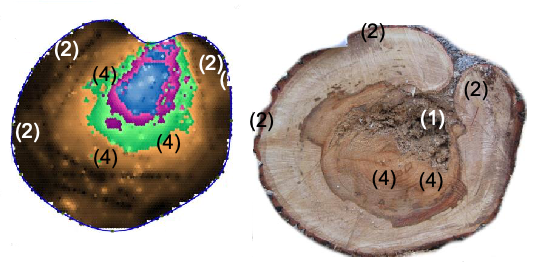
\includegraphics[width=\linewidth]{img/tomograph}
	\caption[Example tomograph visualisation and trunk cross-section photograph]{An example of a sonic tomograph image (left) and across section of
		the same tree (right), annotated to show internal features of the stem:
		(1) cavity or dead dry wood, (2) sound wood, (4) active decay with dense
	wood. Taken from \citet{Picus2016}.}
	\label{legacy:tomograph}
\end{figure}

I aim to test a novel method for estimating the biomass of the largest trees in the 22 plots already covered by the terrestrial LiDAR dataset, using a combination of terrestrial LiDAR and sonic tomography, to map the exterior and interior of the tree, respectively. LiDAR and tomography measurements will be combined with conventional measurements of tree stem diameter, tree height, and wood density, to build a multi-input allometric model of large trees with the hope of further reducing the large uncertainty in the woody biomass stocks of southern African woodlands. Additionally, the new biomass estimations will be compared to biomass estimates generated from existing allometric equations for dry tropical trees, e.g. \citet{Chave2014} and \citet{Ryan2011}, to assess whether these allometries produce an over- or under-estimation of biomass. Specifically, I propose to use the PiCUS 3 sonic tomograph with the protocol outlined in \citet{Gilbert2016} to measure internal structure, and the pipe-fitting algorithm from \citet{Calders2014} to create 3D branch models of exterior structure. Ideally the fieldwork for this project could be carried out alongside a repeat census of the permanent plots, which in Bicuar National Park will happen in either 2022 or 2023, taking advantage of the existing plot monitoring infrastructure and existing LiDAR data.

\subsection{Effects of canopy structure on understorey light environment and grass biomass}
\label{legacy:ssec:grass}

The competitive balance between grass and trees defines mesic savanna ecosystems \citep{Frost1996}. Where rainfall does not preclude a closed tree canopy \citep{Sankaran2005}, disturbance by fire can prevent canopy closure via a positive feedback loop whereby an open canopy allows grass growth, providing fuel for more frequent and intense fires, causing tree mortality, particularly among juveniles, preventing canopy closure, and so on \citep{Staver2011}. This positive feedback drives the phenomenon of `alternative stable states', where nearby and environmentally similar patches can maintain different vegetation based on previous disturbance history. This commonly produces a mosaic of open savanna patches and closed canopy forest-like patches. 

Much previous research has tried to identify the factors which determine the spatial patterning of closed and open canopy patches in mesic savannas, and particularly the factors determining the resilience of patches to state transitions \citep{Devine2017, Case2016, Hirota2011}. Of particular interest has been the transition from open savanna to a closed canopy forest-like state, as evidence suggests that atmospheric carbon fertilisation may be driving woody encroachment and woody thickening across mesic savannas \citep{Stevens2017}. Most previous work has focussed on climatic \citep{Case2020}, edaphic \citep{Colgan2012} and disturbance factors \citep{Case2016}, and how these interact with tree and grass growth to determine their competitive balance, but few have considered biotic factors such as tree demographic structure, canopy architecture and tree species composition (but see \citealt{Pilon2020}), which may also influence grass growth \citep{Jennings1999}. The LiDAR data collected during this PhD provides a unique opportunity to investigate the relationship between canopy tree attributes and grass biomass, to draw conclusions about the tree canopy conditions which provide resilience in open and closed canopy states.

Although the data was not included in the thesis due to lack of time for analysis, the terrestrial LiDAR dataset collected in Bicuar National Park was paired with systematic grass biomass harvest samples and grass sward height measurements using a Disc Pasture Meter (DPM), across all 15 plots (\autoref{legacy:subplot}). \citet{Cooper2017} provides a method for estimating grass volume from terrestrial LiDAR, which could be extended in this study to estimate grass biomass through an allometric equation linking grass volume to sward height and biomass harvests. The sample locations of the grass measurements are precisely known from differential-GPS and can therefore be matched precisely with the LiDAR measurements, providing data on canopy structure at the fine spatial scale relevant to grass growth. 

Using simple linear mixed effects models to explore the relative importance of different tree canopy architectural and structural properties, these data could be used to improve our understanding the drivers of woody encroachment and alternative stable states, which could be applied to earth system models at regional spatial scales to predict how resilient different vegetation types are to environmental change, with consequences for biomass and carbon cycling predictions.

\begin{figure}
	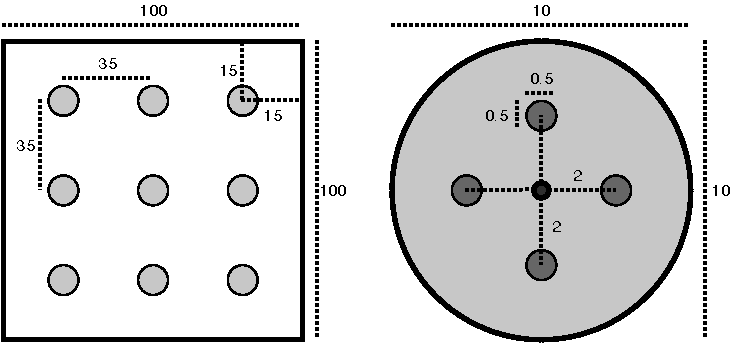
\includegraphics[width=\linewidth]{img/subplot}
	\caption[Grass biomass harvesting subplot layout]{The layout of 10 m diameter subplots within each 1 ha square plot. Distances are marked by dotted lines, in metres. Each subplot is situated inside a 15 m buffer from the plot edge, with 35 m between subplot centres. Subplots are arranged in a 3x3 grid. Disc Pasture Measurements (DPM) and biomass samples are located in cardinal directions 2 m from the centre of the subplot. All distances are in metres. Biomass harvests were conducted at one randomly selected DPM sample point per subplot, resulting in nine biomass harvests and 36 DPM samples per 1 ha plot.}
	\label{legacy:subplot}
\end{figure}

\newpage{}
\FloatBarrier{}
\begingroup
\setstretch{1.0}
\printbibliography[heading=subbibintoc]
\endgroup

\end{refsection}

